Let us consider the BCS Hamiltonian
\begin{equation*}
	H = \sum_{k \sigma} \xi_k c_{k \sigma} \D c_{k \sigma} +  \frac{1}{\Omega} \sum_{k, k'} V_{k k'} c\D_{k' \up} c\D_{-k' \down} c_{-k \down} c_{k \up},
\end{equation*}
where $\xi_k = \varepsilon_k - \mu$ is the single particle energy with respect to the chemical potential $\mu$. We introduce the creation operators for Bogoliubov quasiparticles, denoted $\gamma_{k \sigma}\D$, via the Bogoliubov rotation
\begin{equation*}
	\begin{pmatrix}
		\gamma_{k \up} \\ \gamma_{-k\down}\D
	\end{pmatrix}
	=
	\begin{pmatrix}
	    \sin \theta_k & -\cos \theta_k \\
	    \cos \theta_k & \sin \theta_k \\
	\end{pmatrix}
	\begin{pmatrix}
		c_{k \up} \\ c_{-k \down}
	\end{pmatrix},
	\hspace{10 mm} 
	\tan \theta_k = \frac{\Delta_k}{E_k - \xi_k},
\end{equation*}
where $\Delta_k = - \frac{1}{\Omega} \sum_k V_{kk'} \langle c_{-k \down} c_{k' \up}\rangle$ is the gap function and $E_k = \sqrt{\Delta_k^2 + \xi_k^2}$. It's usefull to have
\begin{equation*}
	\begin{pmatrix}
		c_{k \up} \\ c_{-k \down}
	\end{pmatrix} = \begin{pmatrix}
	    \sin \theta_k & \cos \theta_k \\
	    -\cos \theta_k & \sin \theta_k \\
	\end{pmatrix}
	\begin{pmatrix}
		\gamma_{k \up} \\ \gamma_{-k \down}\D
	\end{pmatrix} = 
	\begin{pmatrix}
	    u_p & v_p \\
	    0 & 0 \\
	\end{pmatrix}
	\begin{pmatrix}
		\gamma_{k \up} \\ \gamma_{-k \down}\D
	\end{pmatrix}
\end{equation*}

The Bogoliubov quasiparticles satisfy the usual fermionic anti-commutation
relations \textbf{(1)}:
\begin{align*}
	\left\{\gamma_{k \up}, \gamma_{k' \down}\right\} &= \sin \theta_k \cos \theta_{-k'} \delta_{k,-k'} - \cos \theta_k \sin \theta_{-k'} \delta_{k, -k'} = 0, \\
	\{\gamma_{k \sigma}, \gamma_{k' \sigma'}\} &= \left\{
		\sin \theta_k c_{k \up} - \cos \theta_k c_{-k \down}\D,
		\ 
		\sin \theta_{k'} c_{k' \up} - \cos \theta_{k'} c_{-k' \down}\D
	\right\} = 0, \\
	\left\{ 
		\gamma_{k \up}, \ \gamma_{k' \up}\D
	\right\} &= \sin \theta_k \sin \theta_{k'} \delta_{k k'} + \cos \theta_k \cos \theta_{k'} \delta_{k k'} = \delta_{k k'}.
\end{align*}

\textbf{Hamiltonian}. In the mean-field approximation, the BCS Hamiltonian takes the form
\begin{equation*}
	H \approx \sum_{k \sigma} \xi_k c_{k \sigma}\D c_{k \sigma} -
	 \sum_k \left(
	 	\Delta_k c\D_{k \up}c_{-k\down}\D + \bar{\Delta}_k c_{-k \down} c_{k \up} + \const
	 \right),
\end{equation*}
introducing operators of the form
\begin{equation*}
A_k \overset{\mathrm{def}}{=} c_{k \up}\D c_{-k \down}\D,
\hspace{10 mm} 
B_k \overset{\mathrm{def}}{=} c_{-k \down} c_{k \up},
\end{equation*}
 the mean-field approximation
amounts to approximating
\begin{equation*}
	\left(A_{k'} - \langle A_{k'}\rangle\right)(B_{k} - \langle B_k\rangle) \approx 0,
\end{equation*}
i.e. neglecting fluctuations around
the expectation values in quadratic order. 
The interaction \textbf{(2)}
\begin{align*}
	V = \frac{1}{\Omega} \sum_{k k'} V_{k k'}  A_{k'} B_{k} &= 
	\frac{1}{\Omega} \sum_{k k'} A_{k'} \langle B_k\rangle + \frac{1}{\Omega} \sum_{k k'} V_{k k'} \langle A_k'\rangle B_k - \frac{1}{\Omega} \sum_{k k'} \langle A_{k'}\rangle \langle B_{k}\rangle 
	\\
	&= - \sum_{k'} \Delta_{k'} A_{k'} - \sum_k \bar{\Delta}_k B_{k} + \const.
\end{align*}



Moving on to quasiparticles, we find \textbf{(3)}
\begin{align*}
	H &= \sum_k \begin{pmatrix}
		c_{k \up}\D & c_{-k \down}
	\end{pmatrix}
	 \begin{pmatrix}
	     \xi_k & -\Delta_k \\
	     -\Delta_k & \xi_k \\
	 \end{pmatrix}
	 \begin{pmatrix}
	 	c_{k \up} \\ c_{-k \down}\D
	 \end{pmatrix} + \const \\
	 &= \sum_k \begin{pmatrix}
	 	\gamma_{k \up}\D & \gamma_{-k \down} 
	 \end{pmatrix} \begin{pmatrix}
	    \sin \theta_k & \cos \theta_k \\
	    -\cos \theta_k & \sin \theta_k \\
	\end{pmatrix}  \begin{pmatrix}
	     \xi_k & -\Delta_k \\
	     -\Delta_k & \xi_k \\
	 \end{pmatrix} 
	 \begin{pmatrix}
	    \sin \theta_k & -\cos \theta_k \\
	    \cos \theta_k & \sin \theta_k \\
	\end{pmatrix}
	\begin{pmatrix}
		\gamma_{k \up} \\ \gamma_{-k \down}\D
	\end{pmatrix} + \const
	\\ 
	&\overset{\mathrm{?}}{=}  \sum_k \begin{pmatrix}
	 	\gamma_{k \up}\D & \gamma_{-k \down} 
	 \end{pmatrix} 
	 \begin{pmatrix}
	     \tilde{E}_k & 0 \\
	     0 & -\tilde{E}_k \\
	 \end{pmatrix}
	\begin{pmatrix}
		\gamma_{k \up} \\ \gamma_{-k \down}\D
	\end{pmatrix},
\end{align*}
with 
\begin{equation*}
	\tilde{E}_k =\xi_k  - 2 \xi_k \cos(\theta_k)^2 + 2 \Delta_k \sin \theta_k \cos \theta_k = \frac{\xi_k^2 + \Delta_k^2}{E_k} = E_k.
\end{equation*}
With $\Delta_k = \Delta$  we could plot the dispersion relation (fig. \ref{fig:131}).

\begin{figure}[t]
    \centering
    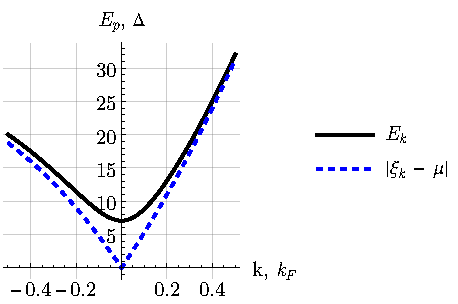
\includegraphics{imgs/MB132.pdf}
    \caption{The dispersion relation}
    \label{fig:131}
\end{figure}


\textbf{Ground state}. The BCS state
\begin{equation*}
	\gs = \prod_k \left(
		\sin \theta_k + \cos \theta_k c_{k \up}\D c_{-k \down}\D
	\right) \ket{0},
\end{equation*}
has zero Bogoliubov quasiparticles \textbf{(4)}:
\begin{align*}
	\gamma_{k \up} \gs &= \left(\sin \theta_k c_{k \up} - \cos \theta_k c_{-k \down}\D\right) \prod_k \left(
		\sin \theta_k + \cos \theta_k c_{k \up}\D c_{-k \down}\D
	\right) \ket{0} 
	\\&= \sin \theta_k c_{k \up} c_{k\up}\D c_{-k\down}\D \ket{0} - \cos \theta_k \sin \theta_k c_{-k\down}\D \ket{0} = 0,
\end{align*}
so $\gs$ is ground state of the mean field approximation of $H$. Actually the $\gs$ could be observed by
\begin{equation*}
	\gs \overset{\mathrm{n}}{=} \prod_{k} \gamma_{-k \down} \gamma_{k \down} \ket{0}.
\end{equation*}

In this state
\begin{equation*}
	E(\theta_k) = \bk{\text{gs}}[H]{\text{gs}} = \sum_k 2 \xi_k \cos^2 \theta_k + \frac{1}{4\Omega} \sum_{k k'} V_{kk'} \sin(2 \theta_k) \sin(2 \theta_{k'}),
\end{equation*}
and we could find $\theta_k$ just by minimizing the energy
\begin{equation*}
	\frac{\partial }{\partial \theta_q} E(\theta_k) = \frac{1}{\Omega}\cos(2 \theta_q) \sum_k V_{qk} \sin(2 \theta_k) - 2 \xi_q \sin(2 \theta_q) = 0.
\end{equation*}
Using this relation we could simplify expression \textbf{(5)}
\begin{equation*}
	\Delta_k = - \frac{1}{\Omega} \sum_{k'} V_{k k'} \langle c_{-k' \down} c_{k' \up} \rangle_{\text{gs}} = - \frac{1}{2\Omega}\sum_{k'}  V_{kk'} \sin(2 \theta_{k'}) = 
	- \frac{1}{\Omega} \sum_{k'} V_{k k'} \frac{\Delta_{k'}}{2 E_{k'}},
\end{equation*}
the zero temperature gap equation.








% and
% \begin{equation*}
% 		\hspace{5 mm} 
% 	\Leftarrow
% 	\hspace{5 mm} 
% 	\left\{c_{k \up}, c_{k' \up}\right\} = 0,
% 	 \ 
% 	\left\{c_{k \up}, c_{-k' \down}\right\} = 0,
% 	\ \ldots
% \end{equation*}